\documentclass[aspectratio=169,11pt,t]{beamer}
\usepackage{tikz}
\setbeamertemplate{navigation symbols}{}
\setbeamertemplate{footline}{\hbox to \paperwidth{\hspace*{8mm}\tiny Deck \hfill
  \foreach \p [count=\i] in {One,Two,Three}{\ifnum\i=\value{section}\textbf{\p}\else\p\fi\hspace{3mm}}%
  \hfill\insertframenumber/\inserttotalframenumber\hspace*{8mm}}\vskip 3mm}
\begin{document}
\section{Part 1}
\begin{frame}{Frame 1}
\begin{itemize}
\item Point one of frame 1, with some words to break a line or two in the column.
\item<2-> Point two, shown on the second overlay.
\end{itemize}
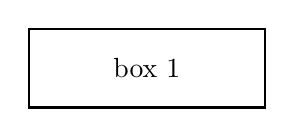
\begin{tikzpicture}\draw[thick] (0,0) rectangle (3,1) node[midway] {box 1};\end{tikzpicture}
\end{frame}

\begin{frame}{Rows 2}
\begin{center}
\uncover<1->{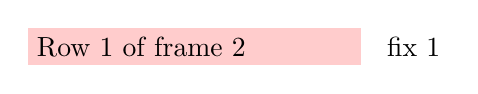
\begin{tikzpicture}\node[fill=red!20,text width=4cm] (s) {Row 1 of frame 2};\node[anchor=west] at ([xshift=2mm]s.east) {fix 1};\end{tikzpicture}}\par
\uncover<2->{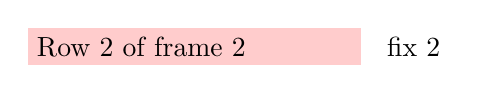
\begin{tikzpicture}\node[fill=red!20,text width=4cm] (s) {Row 2 of frame 2};\node[anchor=west] at ([xshift=2mm]s.east) {fix 2};\end{tikzpicture}}\par
\uncover<3->{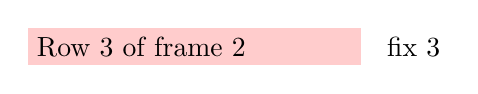
\begin{tikzpicture}\node[fill=red!20,text width=4cm] (s) {Row 3 of frame 2};\node[anchor=west] at ([xshift=2mm]s.east) {fix 3};\end{tikzpicture}}\par
\uncover<4->{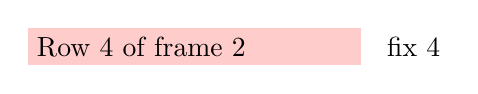
\begin{tikzpicture}\node[fill=red!20,text width=4cm] (s) {Row 4 of frame 2};\node[anchor=west] at ([xshift=2mm]s.east) {fix 4};\end{tikzpicture}}\par
\uncover<5->{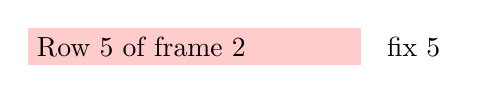
\begin{tikzpicture}\node[fill=red!20,text width=4cm] (s) {Row 5 of frame 2};\node[anchor=west] at ([xshift=2mm]s.east) {fix 5};\end{tikzpicture}}\par
\end{center}
\end{frame}

\begin{frame}{Frame 2}
\begin{itemize}
\item Point one of frame 2, with some words to break a line or two in the column.
\item<2-> Point two, shown on the second overlay.
\end{itemize}
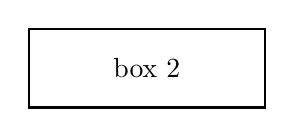
\begin{tikzpicture}\draw[thick] (0,0) rectangle (3,1) node[midway] {box 2};\end{tikzpicture}
\end{frame}

\begin{frame}{Frame 3}
\begin{itemize}
\item Point one of frame 3, with some words to break a line or two in the column.
\item<2-> Point two, shown on the second overlay.
\end{itemize}
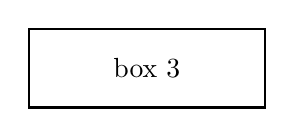
\begin{tikzpicture}\draw[thick] (0,0) rectangle (3,1) node[midway] {box 3};\end{tikzpicture}
\end{frame}

{\setbeamercolor{background canvas}{bg=blue!30!black}
\begin{frame}[plain]
\begin{tikzpicture}[remember picture,overlay]
  \node[font=\Huge,text=white] at ([yshift=10mm]current page.center) {Dark 4};
  \node[text=yellow] at ([yshift=-10mm]current page.center) {A line under it.};
\end{tikzpicture}
\end{frame}}

\begin{frame}{Rows 4}
\begin{center}
\uncover<1->{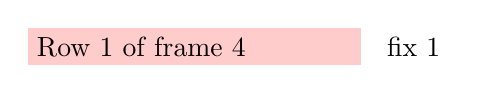
\begin{tikzpicture}\node[fill=red!20,text width=4cm] (s) {Row 1 of frame 4};\node[anchor=west] at ([xshift=2mm]s.east) {fix 1};\end{tikzpicture}}\par
\uncover<2->{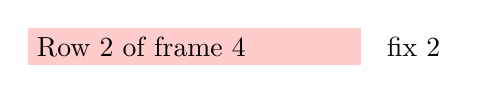
\begin{tikzpicture}\node[fill=red!20,text width=4cm] (s) {Row 2 of frame 4};\node[anchor=west] at ([xshift=2mm]s.east) {fix 2};\end{tikzpicture}}\par
\uncover<3->{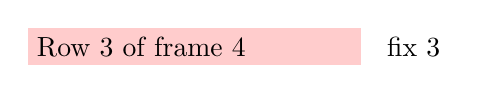
\begin{tikzpicture}\node[fill=red!20,text width=4cm] (s) {Row 3 of frame 4};\node[anchor=west] at ([xshift=2mm]s.east) {fix 3};\end{tikzpicture}}\par
\uncover<4->{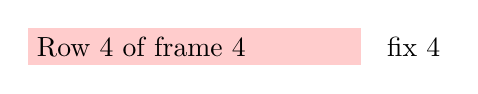
\begin{tikzpicture}\node[fill=red!20,text width=4cm] (s) {Row 4 of frame 4};\node[anchor=west] at ([xshift=2mm]s.east) {fix 4};\end{tikzpicture}}\par
\uncover<5->{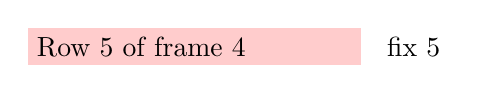
\begin{tikzpicture}\node[fill=red!20,text width=4cm] (s) {Row 5 of frame 4};\node[anchor=west] at ([xshift=2mm]s.east) {fix 5};\end{tikzpicture}}\par
\end{center}
\end{frame}

\begin{frame}{Frame 5}
\begin{itemize}
\item Point one of frame 5, with some words to break a line or two in the column.
\item<2-> Point two, shown on the second overlay.
\end{itemize}
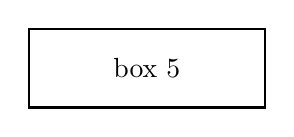
\begin{tikzpicture}\draw[thick] (0,0) rectangle (3,1) node[midway] {box 5};\end{tikzpicture}
\end{frame}

\begin{frame}{Frame 6}
\begin{itemize}
\item Point one of frame 6, with some words to break a line or two in the column.
\item<2-> Point two, shown on the second overlay.
\end{itemize}
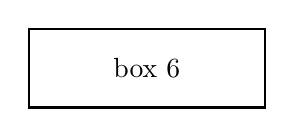
\begin{tikzpicture}\draw[thick] (0,0) rectangle (3,1) node[midway] {box 6};\end{tikzpicture}
\end{frame}

\begin{frame}{Rows 6}
\begin{center}
\uncover<1->{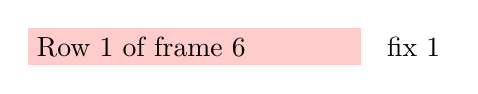
\begin{tikzpicture}\node[fill=red!20,text width=4cm] (s) {Row 1 of frame 6};\node[anchor=west] at ([xshift=2mm]s.east) {fix 1};\end{tikzpicture}}\par
\uncover<2->{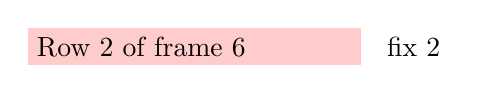
\begin{tikzpicture}\node[fill=red!20,text width=4cm] (s) {Row 2 of frame 6};\node[anchor=west] at ([xshift=2mm]s.east) {fix 2};\end{tikzpicture}}\par
\uncover<3->{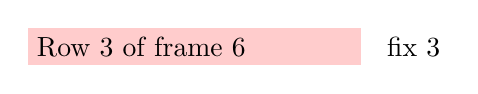
\begin{tikzpicture}\node[fill=red!20,text width=4cm] (s) {Row 3 of frame 6};\node[anchor=west] at ([xshift=2mm]s.east) {fix 3};\end{tikzpicture}}\par
\uncover<4->{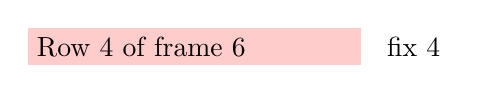
\begin{tikzpicture}\node[fill=red!20,text width=4cm] (s) {Row 4 of frame 6};\node[anchor=west] at ([xshift=2mm]s.east) {fix 4};\end{tikzpicture}}\par
\uncover<5->{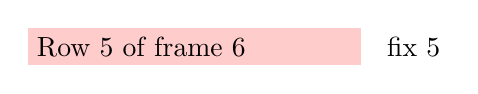
\begin{tikzpicture}\node[fill=red!20,text width=4cm] (s) {Row 5 of frame 6};\node[anchor=west] at ([xshift=2mm]s.east) {fix 5};\end{tikzpicture}}\par
\end{center}
\end{frame}

\begin{frame}{Frame 7}
\begin{itemize}
\item Point one of frame 7, with some words to break a line or two in the column.
\item<2-> Point two, shown on the second overlay.
\end{itemize}
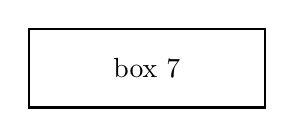
\begin{tikzpicture}\draw[thick] (0,0) rectangle (3,1) node[midway] {box 7};\end{tikzpicture}
\end{frame}

\section{Part 8}
{\setbeamercolor{background canvas}{bg=blue!30!black}
\begin{frame}[plain]
\begin{tikzpicture}[remember picture,overlay]
  \node[font=\Huge,text=white] at ([yshift=10mm]current page.center) {Dark 8};
  \node[text=yellow] at ([yshift=-10mm]current page.center) {A line under it.};
\end{tikzpicture}
\end{frame}}

\begin{frame}{Frame 9}
\begin{itemize}
\item Point one of frame 9, with some words to break a line or two in the column.
\item<2-> Point two, shown on the second overlay.
\end{itemize}
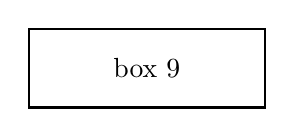
\begin{tikzpicture}\draw[thick] (0,0) rectangle (3,1) node[midway] {box 9};\end{tikzpicture}
\end{frame}

\begin{frame}{Rows 8}
\begin{center}
\uncover<1->{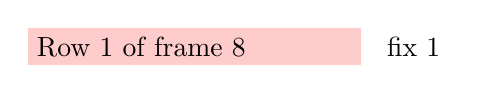
\begin{tikzpicture}\node[fill=red!20,text width=4cm] (s) {Row 1 of frame 8};\node[anchor=west] at ([xshift=2mm]s.east) {fix 1};\end{tikzpicture}}\par
\uncover<2->{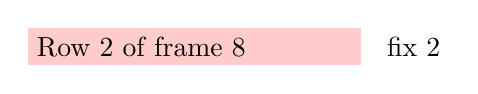
\begin{tikzpicture}\node[fill=red!20,text width=4cm] (s) {Row 2 of frame 8};\node[anchor=west] at ([xshift=2mm]s.east) {fix 2};\end{tikzpicture}}\par
\uncover<3->{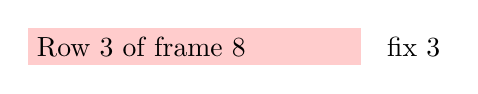
\begin{tikzpicture}\node[fill=red!20,text width=4cm] (s) {Row 3 of frame 8};\node[anchor=west] at ([xshift=2mm]s.east) {fix 3};\end{tikzpicture}}\par
\uncover<4->{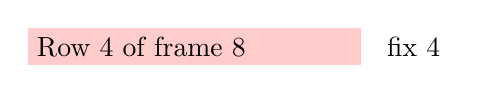
\begin{tikzpicture}\node[fill=red!20,text width=4cm] (s) {Row 4 of frame 8};\node[anchor=west] at ([xshift=2mm]s.east) {fix 4};\end{tikzpicture}}\par
\uncover<5->{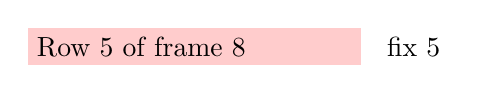
\begin{tikzpicture}\node[fill=red!20,text width=4cm] (s) {Row 5 of frame 8};\node[anchor=west] at ([xshift=2mm]s.east) {fix 5};\end{tikzpicture}}\par
\end{center}
\end{frame}

\begin{frame}{Frame 10}
\begin{itemize}
\item Point one of frame 10, with some words to break a line or two in the column.
\item<2-> Point two, shown on the second overlay.
\end{itemize}
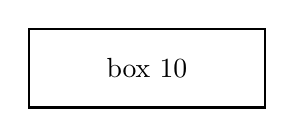
\begin{tikzpicture}\draw[thick] (0,0) rectangle (3,1) node[midway] {box 10};\end{tikzpicture}
\end{frame}

\begin{frame}{Frame 11}
\begin{itemize}
\item Point one of frame 11, with some words to break a line or two in the column.
\item<2-> Point two, shown on the second overlay.
\end{itemize}
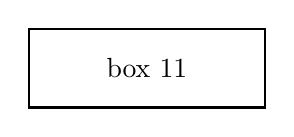
\begin{tikzpicture}\draw[thick] (0,0) rectangle (3,1) node[midway] {box 11};\end{tikzpicture}
\end{frame}

{\setbeamercolor{background canvas}{bg=blue!30!black}
\begin{frame}[plain]
\begin{tikzpicture}[remember picture,overlay]
  \node[font=\Huge,text=white] at ([yshift=10mm]current page.center) {Dark 12};
  \node[text=yellow] at ([yshift=-10mm]current page.center) {A line under it.};
\end{tikzpicture}
\end{frame}}

\begin{frame}{Rows 10}
\begin{center}
\uncover<1->{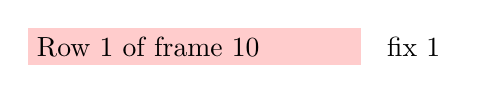
\begin{tikzpicture}\node[fill=red!20,text width=4cm] (s) {Row 1 of frame 10};\node[anchor=west] at ([xshift=2mm]s.east) {fix 1};\end{tikzpicture}}\par
\uncover<2->{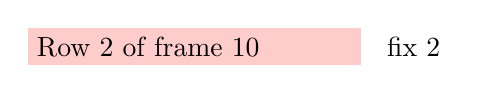
\begin{tikzpicture}\node[fill=red!20,text width=4cm] (s) {Row 2 of frame 10};\node[anchor=west] at ([xshift=2mm]s.east) {fix 2};\end{tikzpicture}}\par
\uncover<3->{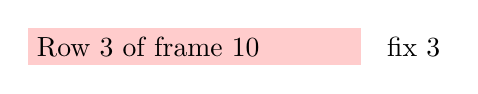
\begin{tikzpicture}\node[fill=red!20,text width=4cm] (s) {Row 3 of frame 10};\node[anchor=west] at ([xshift=2mm]s.east) {fix 3};\end{tikzpicture}}\par
\uncover<4->{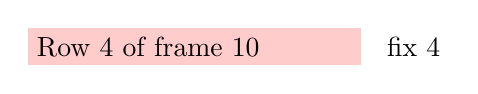
\begin{tikzpicture}\node[fill=red!20,text width=4cm] (s) {Row 4 of frame 10};\node[anchor=west] at ([xshift=2mm]s.east) {fix 4};\end{tikzpicture}}\par
\uncover<5->{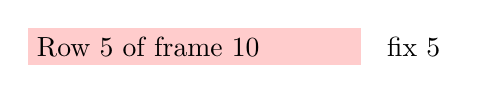
\begin{tikzpicture}\node[fill=red!20,text width=4cm] (s) {Row 5 of frame 10};\node[anchor=west] at ([xshift=2mm]s.east) {fix 5};\end{tikzpicture}}\par
\end{center}
\end{frame}

\begin{frame}{Frame 13}
\begin{itemize}
\item Point one of frame 13, with some words to break a line or two in the column.
\item<2-> Point two, shown on the second overlay.
\end{itemize}
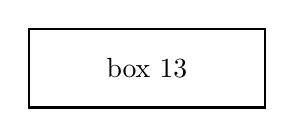
\begin{tikzpicture}\draw[thick] (0,0) rectangle (3,1) node[midway] {box 13};\end{tikzpicture}
\end{frame}

\begin{frame}{Frame 14}
\begin{itemize}
\item Point one of frame 14, with some words to break a line or two in the column.
\item<2-> Point two, shown on the second overlay.
\end{itemize}
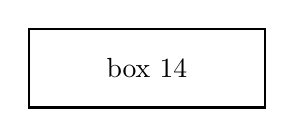
\begin{tikzpicture}\draw[thick] (0,0) rectangle (3,1) node[midway] {box 14};\end{tikzpicture}
\end{frame}

\section{Part 15}
\begin{frame}{Rows 12}
\begin{center}
\uncover<1->{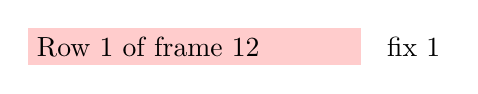
\begin{tikzpicture}\node[fill=red!20,text width=4cm] (s) {Row 1 of frame 12};\node[anchor=west] at ([xshift=2mm]s.east) {fix 1};\end{tikzpicture}}\par
\uncover<2->{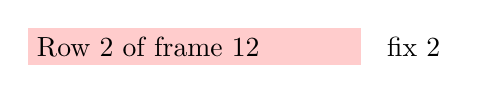
\begin{tikzpicture}\node[fill=red!20,text width=4cm] (s) {Row 2 of frame 12};\node[anchor=west] at ([xshift=2mm]s.east) {fix 2};\end{tikzpicture}}\par
\uncover<3->{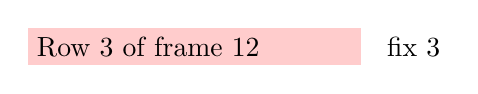
\begin{tikzpicture}\node[fill=red!20,text width=4cm] (s) {Row 3 of frame 12};\node[anchor=west] at ([xshift=2mm]s.east) {fix 3};\end{tikzpicture}}\par
\uncover<4->{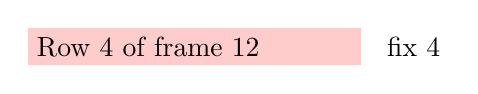
\begin{tikzpicture}\node[fill=red!20,text width=4cm] (s) {Row 4 of frame 12};\node[anchor=west] at ([xshift=2mm]s.east) {fix 4};\end{tikzpicture}}\par
\uncover<5->{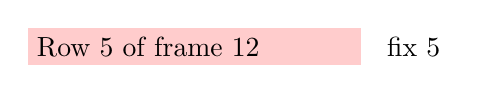
\begin{tikzpicture}\node[fill=red!20,text width=4cm] (s) {Row 5 of frame 12};\node[anchor=west] at ([xshift=2mm]s.east) {fix 5};\end{tikzpicture}}\par
\end{center}
\end{frame}

\begin{frame}{Frame 15}
\begin{itemize}
\item Point one of frame 15, with some words to break a line or two in the column.
\item<2-> Point two, shown on the second overlay.
\end{itemize}
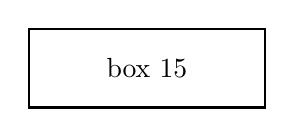
\begin{tikzpicture}\draw[thick] (0,0) rectangle (3,1) node[midway] {box 15};\end{tikzpicture}
\end{frame}

{\setbeamercolor{background canvas}{bg=blue!30!black}
\begin{frame}[plain]
\begin{tikzpicture}[remember picture,overlay]
  \node[font=\Huge,text=white] at ([yshift=10mm]current page.center) {Dark 16};
  \node[text=yellow] at ([yshift=-10mm]current page.center) {A line under it.};
\end{tikzpicture}
\end{frame}}

\begin{frame}{Frame 17}
\begin{itemize}
\item Point one of frame 17, with some words to break a line or two in the column.
\item<2-> Point two, shown on the second overlay.
\end{itemize}
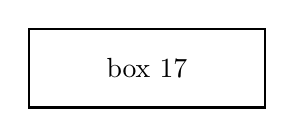
\begin{tikzpicture}\draw[thick] (0,0) rectangle (3,1) node[midway] {box 17};\end{tikzpicture}
\end{frame}

\begin{frame}{Rows 14}
\begin{center}
\uncover<1->{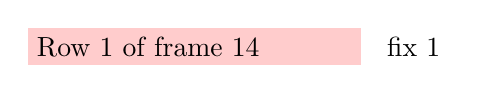
\begin{tikzpicture}\node[fill=red!20,text width=4cm] (s) {Row 1 of frame 14};\node[anchor=west] at ([xshift=2mm]s.east) {fix 1};\end{tikzpicture}}\par
\uncover<2->{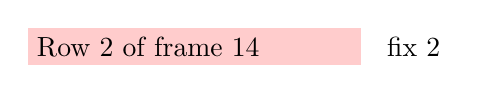
\begin{tikzpicture}\node[fill=red!20,text width=4cm] (s) {Row 2 of frame 14};\node[anchor=west] at ([xshift=2mm]s.east) {fix 2};\end{tikzpicture}}\par
\uncover<3->{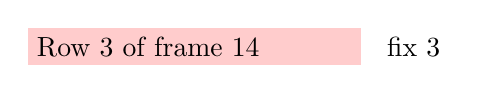
\begin{tikzpicture}\node[fill=red!20,text width=4cm] (s) {Row 3 of frame 14};\node[anchor=west] at ([xshift=2mm]s.east) {fix 3};\end{tikzpicture}}\par
\uncover<4->{\begin{tikzpicture}\node[fill=red!20,text width=4cm] (s) {Row 4 of frame 14};\node[anchor=west] at ([xshift=2mm]s.east) {fix 4};\end{tikzpicture}}\par
\uncover<5->{\begin{tikzpicture}\node[fill=red!20,text width=4cm] (s) {Row 5 of frame 14};\node[anchor=west] at ([xshift=2mm]s.east) {fix 5};\end{tikzpicture}}\par
\end{center}
\end{frame}

\begin{frame}{Frame 18}
\begin{itemize}
\item Point one of frame 18, with some words to break a line or two in the column.
\item<2-> Point two, shown on the second overlay.
\end{itemize}
\begin{tikzpicture}\draw[thick] (0,0) rectangle (3,1) node[midway] {box 18};\end{tikzpicture}
\end{frame}

\begin{frame}{Frame 19}
\begin{itemize}
\item Point one of frame 19, with some words to break a line or two in the column.
\item<2-> Point two, shown on the second overlay.
\end{itemize}
\begin{tikzpicture}\draw[thick] (0,0) rectangle (3,1) node[midway] {box 19};\end{tikzpicture}
\end{frame}

{\setbeamercolor{background canvas}{bg=blue!30!black}
\begin{frame}[plain]
\begin{tikzpicture}[remember picture,overlay]
  \node[font=\Huge,text=white] at ([yshift=10mm]current page.center) {Dark 20};
  \node[text=yellow] at ([yshift=-10mm]current page.center) {A line under it.};
\end{tikzpicture}
\end{frame}}
\end{document}
